%% The following is a directive for TeXShop to indicate the main file
%%!TEX root = ../../thesis.tex

\chapter{Introduction}
\label{ch:introduction}
As conventional, easily accessible, hydrocarbon resources are being depleted, there is an increase in the use of secondary and enhanced recovery techniques, for example using water or CO$_2$ to re-pressurize a reservoir, accompanied by an increase in the exploration and development of unconventional resources such as shale gas formations. The combination of horizontal drilling and hydraulic fracturing are key technologies for extracting hydrocarbons from shale and low permeability, ``tight'' reservoirs. As a byproduct of fracturing, wastewater, if not recycled, must be disposed of. In many cases this is achieved by injecting the wastewater into the subsurface through an injection well. Similarly, with recognition of the hazard that carbon-dioxide poses as a contributor to global warming, efforts are being made to capture and store CO$_2$ in the subsurface. In each of these scenarios, there are both environmental and economic motivations for characterizing the distribution of injected materials.

To focus the research questions addressed in this thesis, we take the application of hydraulic fracturing as the primary motivating application, keeping in mind that the connections and similarities with other subsurface injections.
\section{Hydraulic Fracturing}

Hydraulic fracturing is used to extract hydrocarbons from tight (low-permeability) and shale formations where oil and gas will not easily flow. In such settings, hydraulic fracturing is used to create pathways for the hydrocarbons to flow (Figure \ref{fig:nonconventional_resources}). The process of inducing a fracture involves sealing off a section of the well and pumping fluid into that section under high pressure until the rock fails and cracks open up in the direction of the minimum principal stress. Typically, once the rock has fractured, sand or ceramic particles, referred to as proppant, are pumped into the formation to keep the newly created pathways open. Many of the wells drilled in the past two decades are horizontal wells, and typically 15 to 30 fracture stages (in some cases up to 60) are performed along the length of the well \citep{Maxwell2014}.
The extent of the fractures, and distribution of proppant and fluid within these fractures, are key factors that determine the available pathways for oil or gas to flow to the well, and thus, the resulting production of the resource \citep{Brannon2008, Cipolla2009}. Therefore, in order to assess: how effectively the fracture treatment has stimulated the reservoir, how efficiently resources, such as water, have been used to create the fracture, and to understand the environmental and economic impacts of the fracture itself; we need a method to delineate the extent of the proppant and fluid within the reservoir.


\begin{figure}
    \begin{center}
    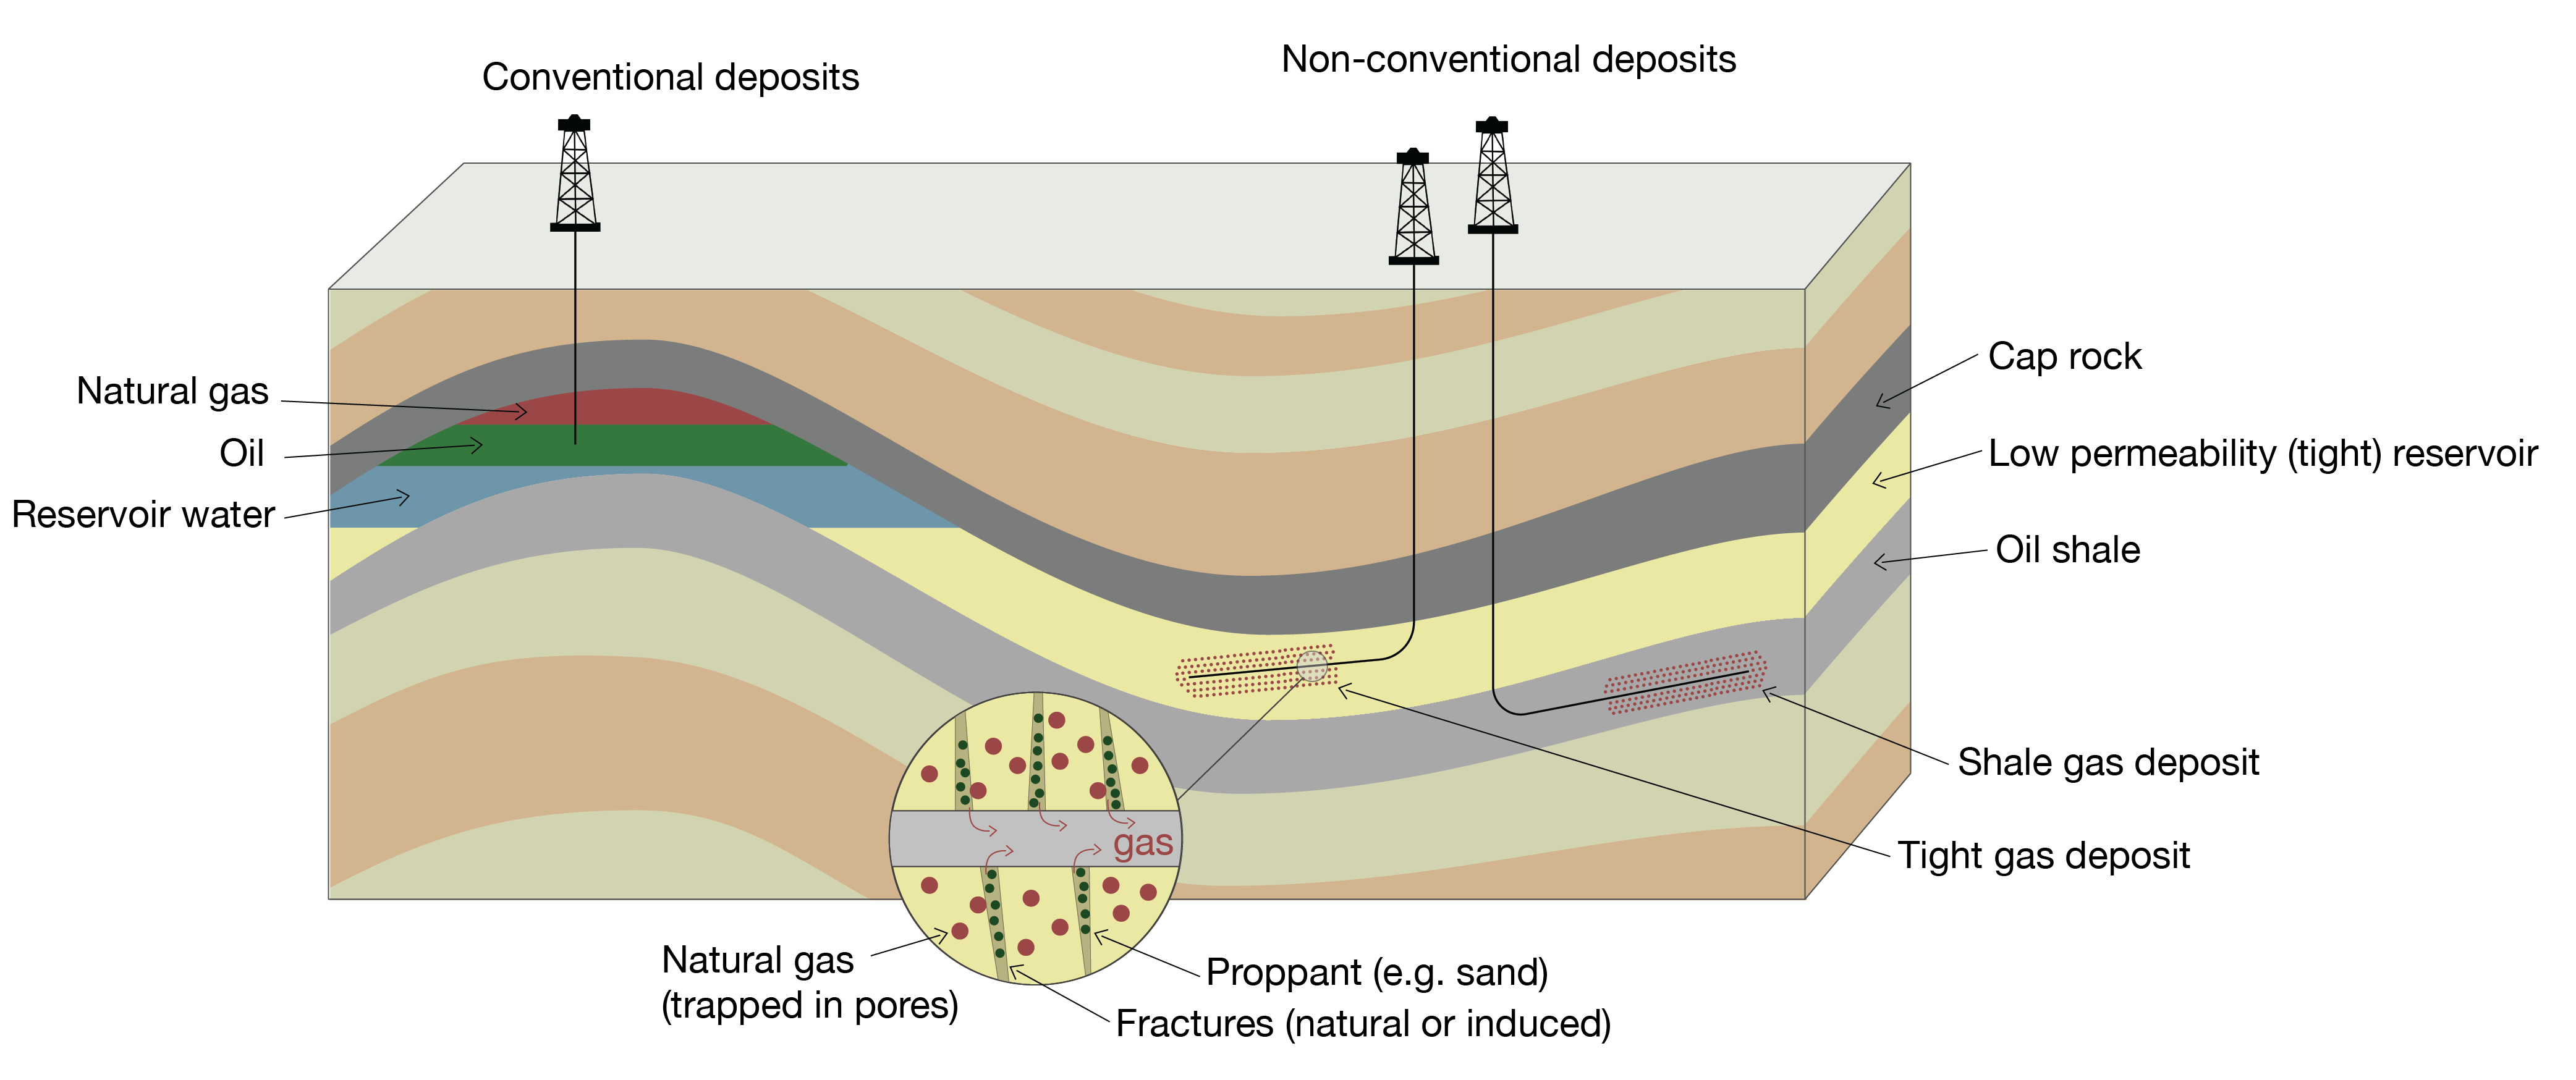
\includegraphics[width=\textwidth]{figures/intro/nonconventional_resources.png}
    \end{center}
\caption{
    Conventional reservoirs contain oil and gas that have migrated upwards
    under pressure until they are trapped by a cap rock (left), while
    non-conventional tight or shale oil and gas reservoirs contain hydrocarbons
    that are trapped in low permeability formations (right).
}
\label{fig:nonconventional_resources}
\end{figure}


Despite recent advances, there are still many unknowns in the fracturing process; chief among them is the extent and distribution of proppant and fluid within the reservoir. Microseismic is used to detect acoustic events generated as the fracture propagates through the reservoir. It can provide information about fracture geometry \citep{Cipolla2009,Warpinski1996,Maxwell2002}, but not all fractures generate a measurable seismic response \citep{Cipolla2000,Barree2002}, and a microseismic response contains no information about the proppant or fluid distribution within the reservoir \citep{Warpinski1996,Barree2002}. Tiltmeters are used to characterize the deformation of the rock due to the presence of a fracture or a change in the stress distribution \citep{Wright1998}, but they are incapable of providing direct information about the proppant or fluid distributions \citep{Cipolla2000,Warpinski1996}. Tracers and well logs are used to characterize the fracture geometry and fluid distribution, but their depth of investigation is limited to within a few meters of the wellbore \citep{Cipolla2000}. To delineate the extent of the proppant within the reservoir, we need a method that is both sensitive to the presence of the injected materials and can be implemented on the reservoir scale \citep{Cipolla2000,Warpinski1996,Barree2002,Cipolla2009}.

To accomplish this task, we propose to use electromagnetic (EM) geophysical techniques. For EM to be a viable method for imaging the distribution of proppant and fluid within a fractured volume of rock, we require that: (1) the fractured volume of rock have physical properties which are distinct from the background, host rock, (2) the survey must be sensitive to this contrast, and (3) once the data have been collected, they must be interpreted or inverted in a meaningful manner. We also note that this is a time-lapse problem; that is, by inducing a fracture, the physical properties of the reservoir have been altered. In order to characterize such a change, we must view the imaging problem as a time-lapse one, and collect data to provide us with a before and an after data-view of the reservoir.

Variations in subsurface electrical conductivity have been used as a diagnostic physical property in sedimentary settings for characterizing geologic formations, and the properties and distribution of fluids within those formations. Hydrocarbons are much more resistive than saline formation fluids. In enhanced oil recovery projects, fluids are injected into the formation, which may be less resistive than the hydrocarbons they replace. These contrasts have been the target of cross-well, surface-to-borehole and borehole-to-surface electromagnetic (EM) methods for reservoir monitoring and characterization applications (cf. \cite{Bevc1991, Wilt1995, marsala2008, marsala2011, marsala2014}).

In the case of hydraulic fracturing, the physical properties of the fractured volume of the reservoir depend upon the properties of the injected fluid and proppant particles. Saline water may be used, as is often the case when recycled water is used, and electrically conductive proppant may be manufactured and injected \citep{cannan2014electrically, Vengosh2014, King2010}. One or both of these may be used to create a physical property contrast between the host reservoir rock and the fractured volume of the reservoir. This contrast is what we aim to excite using an electromagnetic (EM) survey.


\section{Electromagnetic geophysics}

Electromagnetics is governed by Maxwell’s equations,

\begin{equation}
\begin{split}
    \nabla \times \vec{e} + \frac{\partial \vec{b}}{\partial t} &= 0 \\
    \nabla \times \vec{h} - \frac{\partial \vec{d}}{\partial t} &= \vec{j}
\end{split}
\label{eq:maxwell_time_full}
\end{equation}

where $\vec{e}$ is the electric field (V/m), $\vec{b}$ is the magnetic flux density (T), $\vec{h}$ is the magnetic field (A/m), $\vec{d}$ is the electric displacement (C/m$^2$), $\vec{j}$ is the current density (A/m$^2$)


\subsection{Forward simulation}
\section{Geophysical inversions}

Once data have been collected, an inverse problem can be formulated. The goal of the inversion is to extract information about the subsurface from the data. Formulating, implementing and solving the inverse problem can be viewed as a workflow consisting of inputs, implementation, and evaluation, as shown in Figure \ref{fig:inversions}. The inputs are composed of the data, the governing equations , and prior knowledge or assumptions about the setting. In the case of the fracturing problem, this may include well-log resistivity measurements which provide information about the background, knowledge of where the fracture was initiated, and the volumes of proppant and fluid pumped to create the fracture.
The implementation consists of two broad categories: the forward simulation and the inversion. The forward simulation is the means by which we solve the governing equations given a model, and the inversion components evaluate and update this model. We are considering a gradient based approach, which updates the model through an optimization routine. The output of this implementation is a model, which, prior to interpretation, must be evaluated. This requires considering, and often re-assessing, the choices and assumptions made in both the input and implementation stages (c.f. \cite{Oldenburg2005, Haber2014a, Cockett2015}).

\begin{figure}
    \begin{center}
    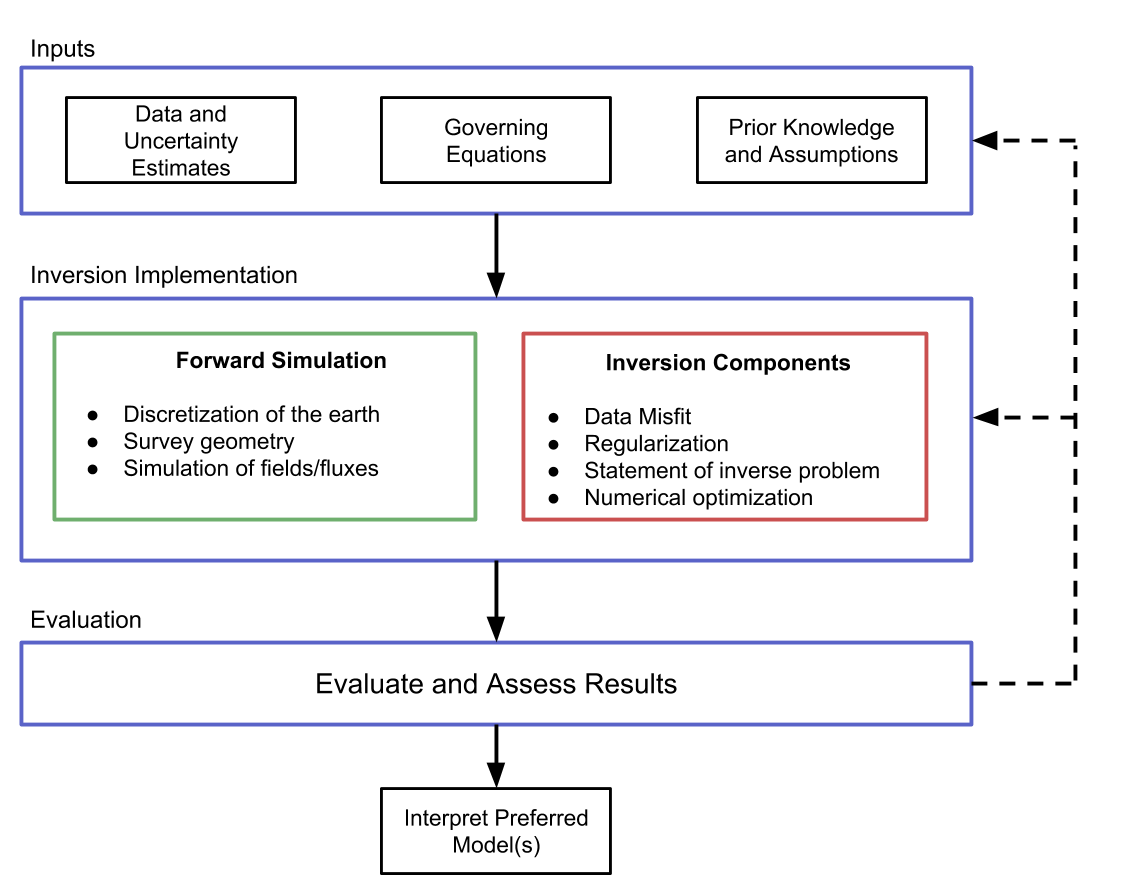
\includegraphics[width=\textwidth]{figures/intro/inversion_workflow_bullets.png}
    \end{center}
\caption{
    Overview of a geophysical inversion workflow. Adapted from \cite{Cockett2015}.
}
\label{fig:inversion_workflow_bullets}
\end{figure}


\section{Steel-cased boreholes}


\section{Thesis outline}

\section{A note on reproducibility}

